\documentclass[a4paper, 9pt]{article}
\usepackage[english,brazil]{babel}
\usepackage[utf8]{inputenc}
\usepackage{fullpage}

\usepackage{multicol, caption}
\setlength{\columnsep}{30pt}

\usepackage{graphicx}
\usepackage{lipsum}
\newenvironment{Figure}
  {\par\medskip\noindent\minipage{\linewidth}}
  {\endminipage\par\medskip}


% Definitions an Theorems: ------------
\usepackage{amsthm}

\theoremstyle{plain}
\newtheorem{statement}{Enunciado}

\theoremstyle{definition}
\newtheorem{explanation}{Explicação}

\theoremstyle{definition}
\newtheorem{discussion}{Discussão}

\theoremstyle{definition}
\newtheorem{answer}{Resposta}
% ----------------------------------------------

% Definitions of languages: ------------
\usepackage{listings}
\lstdefinestyle{cStyle}{
  basicstyle=\scriptsize,
  breakatwhitespace=false,
  breaklines=true,
  captionpos=b,
  keepspaces=true,
  numbers=left,
  numbersep=5pt,
  showspaces=false,
  gobble=4,
  tabsize=4,
  showstringspaces=false,
  showtabs=false,
}
\renewcommand*{\lstlistingname}{Código}

% ----------------------------------------------


\title{Laboratório 3 \\ Otimização com Métodos de Busca Local}
\author{CT-213 \\ Prof. Marcos Ricardo Omena de Albuquerque Maximo  \\ \\ \\  Carlos Matheus Barros da Silva \\carlosmatheusbs@gmail.com \\ \\ \\ \\ \\ \\ \\ \\ \\ \\ \\ \\ \\ \\ \\ \\ \\ \\ \\ \\ \\ \\ \\ \\ \\ \\ \\ \\}
\date{Março - 2019}


\begin{document}

\Huge
\maketitle
\newpage
\normalsize

\begin{multicols}{2}

%-------------------------------------------------------------------------------

\section*{Introdução}

Foram estudados e implementados três métodos de otimização que possuem algoritmos baseados em busca local. Esses métodos foram Gradient Descent, Hill Climbing e Simulated Anneling.

Os métodos foram testados em um problema proposto no roteiro dessa atividade. Esse problema utilizou regressão linear para ober parâmetros físicos relativos ao movimento de uma bola.

Como o problema tratado possui solução analítica, o experimento é a titulo educacional, já que, dessa forma, pode-se obter facilmente sua solução pelo Método dos Mínimos Quadrados (MMQ).

De maneira geral, o Laboratório foi desenvolvido com sucesso. Em cada uma das sessões seguintes encontram-se o respectivo desenvolvimento de um dos métodos estudado.

\section*{Gradient Descent}

\begin{explanation}
    O código para a o algoritmo do Gradient Descent pode ser visto no Código \ref{code:gradient_descent}. Para a implementação desse código foram utilizados, também as funções no Código \ref{code:printhistory} e no Código \ref{code:stopcondition}.

    O resultado desse algoritmo pode ser visto no hitórico de \textit{theta} represetado pelo Código \ref{code:gradient_descent_history} e pode ser visto também na análise da trajetória apresentada na Figura \ref{fig:gradient_descent}.
\end{explanation}

\lstinputlisting[
    language=python,
    caption={Interior da função \textit{Gradient Descent}.},
    label={code:gradient_descent},
    style=cStyle,
    firstline=28,
    lastline=40
]{./../code/gradient_descent.py}
\lstinputlisting[
    language=python,
    caption={Código para criação do arquivo com o hitórico de \textit{theta}.},
    label={code:printhistory},
    style=cStyle,
    firstline=13,
    lastline=18
]{./../code/ball_fit.py}
\lstinputlisting[
    language=python,
    caption={Código para checagem da condição de parada.},
    label={code:stopcondition},
    style=cStyle,
    firstline=21,
    lastline=22
]{./../code/ball_fit.py}
\lstinputlisting[
    language=python,
    caption={Histórico de \textit{theta} para o algoritmo \textit{Gradient Descent} para as 10 primeiras iterações e para as 10 útilmas},
    label={code:gradient_descent_history},
    style=cStyle,
    numbers=none,
    linerange={1-10,993-1002},
]{./../code/gradient_descent.txt}

\begin{Figure}
    \centering
    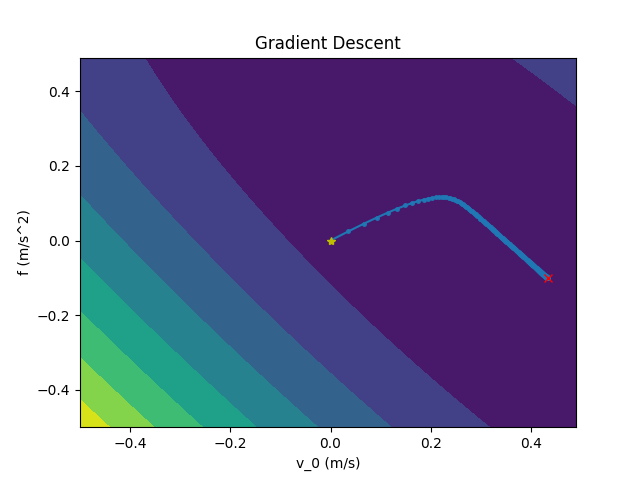
\includegraphics[width=\linewidth]
    {./../code/gradient_descent.png}
    \captionof{figure}{Trajetório com o método \textit{Gradient Descent}.}
    \label{fig:gradient_descent}
\end{Figure}

%-------------------------------------------------------------------------------

\section*{Hill Climbing}

\begin{explanation}
    O código para a o algoritmo do Hill Climbing pode ser visto no Código \ref{code:hill_climbing}. Para a implementação desse código foram utilizados, também as funções no Código \ref{code:printhistory} e no Código \ref{code:stopcondition}.

    O resultado desse algoritmo pode ser visto no hitórico de \textit{theta} represetado pelo Código \ref{code:hill_climbing_history} e pode ser visto também na análise da trajetória apresentada na Figura \ref{fig:hill_climbing}.
\end{explanation}

\lstinputlisting[
    language=python,
    caption={Interior da função \textit{Hill Climbing}.},
    label={code:hill_climbing},
    style=cStyle,
    firstline=26,
    lastline=49
]{./../code/hill_climbing.py}
\lstinputlisting[
    language=python,
    caption={Histórico de \textit{theta} para o algoritmo \textit{Hill Climbing} para as 10 primeiras iterações e para as 10 útilmas},
    label={code:hill_climbing_history},
    style=cStyle,
    numbers=none,
    linerange={1-10,291-300},
]{./../code/hill_climbing.txt}

\begin{Figure}
    \centering
    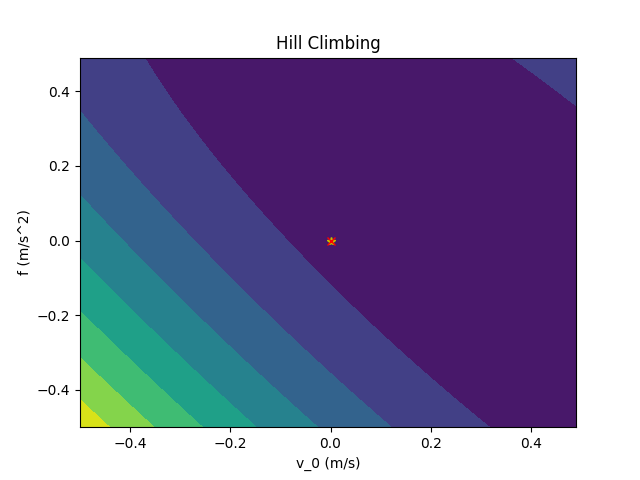
\includegraphics[width=\linewidth]
    {./../code/hill_climbing.png}
    \captionof{figure}{Trajetório com o método \textit{Hill Climbing}.}
    \label{fig:hill_climbing}
\end{Figure}


%-------------------------------------------------------------------------------

\section*{Simulated Anneling}

\begin{explanation}
    O código para a o algoritmo do Simulated Anneling pode ser visto no Código \ref{code:simulated_annealing}. Para a implementação desse código foram utilizados, também as funções no Código \ref{code:printhistory} e no Código \ref{code:stopcondition}.

    O resultado desse algoritmo pode ser visto no hitórico de \textit{theta} represetado pelo Código \ref{code:simulated_annealing_history} e pode ser visto também na análise da trajetória apresentada na Figura \ref{fig:simulated_annealing}.
\end{explanation}

\lstinputlisting[
    language=python,
    caption={Interior da função \textit{Simulated Anneling}.},
    label={code:simulated_annealing},
    style=cStyle,
    firstline=32,
    lastline=57
]{./../code/simulated_annealing.py}
\lstinputlisting[
    language=python,
    caption={Histórico de \textit{theta} para o algoritmo \textit{Simulated Anneling} para as 10 primeiras iterações e para as 10 útilmas},
    label={code:simulated_annealing_history},
    style=cStyle,
    numbers=none,
    linerange={1-10,4991-5000},
]{./../code/simulated_annealing.txt}

\begin{Figure}
    \centering
    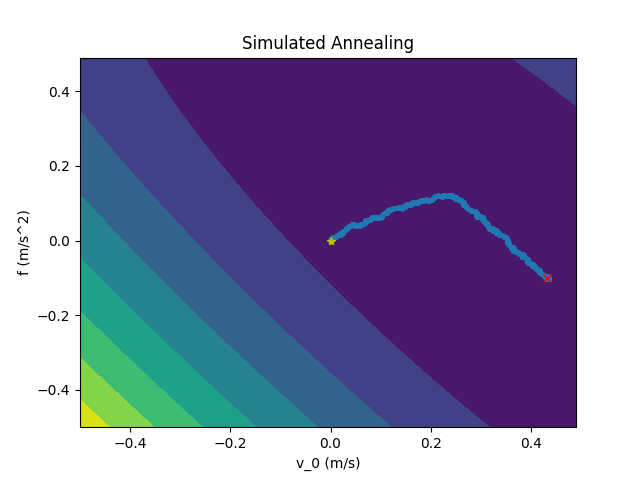
\includegraphics[width=\linewidth]
    {./../code/simulated_annealing.png}
    \captionof{figure}{Trajetório com o método \textit{Simulated Anneling}.}
    \label{fig:simulated_annealing}
\end{Figure}

%-------------------------------------------------------------------------------

\section*{Comparações}

De maneira visual a comparação dos métodos pode ser vista na Figura \ref{fig:curve_fit} e na Figura \ref{fig:comparation}.

Como foi observado o método \textit{Hill Climbing} converge mais rapidamente para um mínimo local, enquanto que o método \textit{Simulated Anneling} converge mais devagar, mas apreseta maior capacidade de encontrar um minimo global ao invez de local. Isso se deve ao fato de que randomicamente ele erra a fim de que possa encontrar outros caminhos.

\begin{Figure}
    \centering
    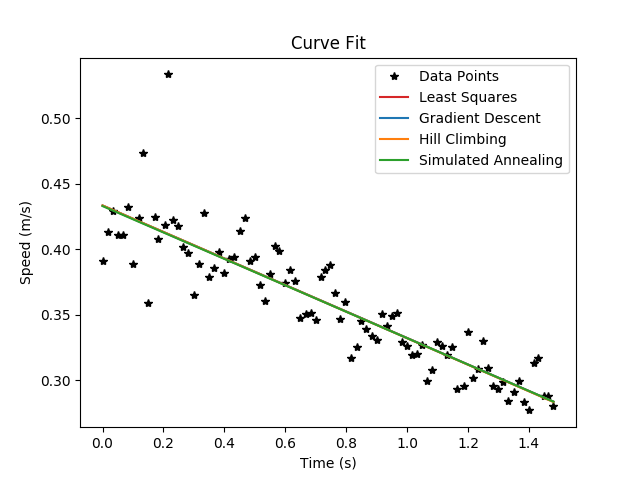
\includegraphics[width=\linewidth]
    {./../code/fit_comparison.png}
    \captionof{figure}{Comparação das cursvas sobre os pontos amostrados.}
    \label{fig:curve_fit}
\end{Figure}

\begin{Figure}
    \centering
    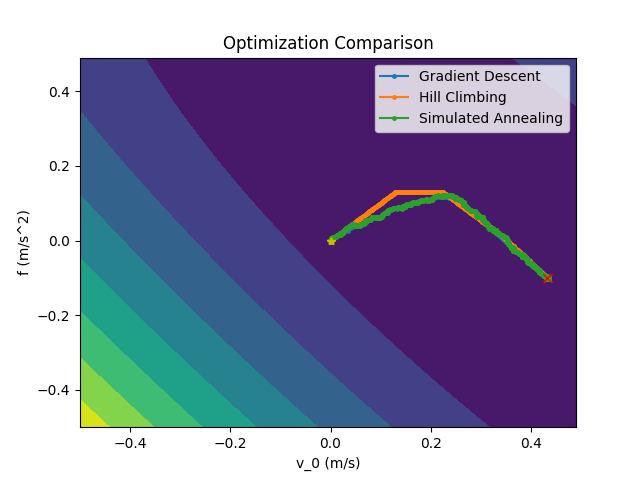
\includegraphics[width=\linewidth]
    {./../code/optimization_comparison.png}
    \captionof{figure}{Comparação das trajetórias entre os métodos}
    \label{fig:comparation}
\end{Figure}


\end{multicols}

\end{document}
